\documentclass{article}
\title{Sars-CoV-2 Epidemiological Analysis with PyCaret ML}
\author{Bryan Alexis Ambriz}
\date{September 2023}
\usepackage[style=authoryear,backend=biber]{biblatex}
\addbibresource{sars_cov_2_epidemiological_analysis_with_pycaret_ml.bib}
\usepackage{graphicx}
\begin{document}
\maketitle
\paragraph{The outbreak of the novel coronavirus, Sars-CoV-2, has led to a global pandemic and posed significant challenges to public health systems worldwide. As a previous research intern at the Scripps Research Institute working with the Andersen Lab, I am in a unique position to apply my skills in epidemiological analysis using PyCaret for machine learning. I am a current graduate student studying Software Engineering and focusing on Data Science, and I am confident that furthering my knowledge in this field can contribute to a comprehensive analysis of Sars-CoV-2.}
\section{\textbf{Business Understanding}}
\paragraph{Our primary business objective is to leverage data analysis and machine learning to identify potential virus lineages that increase transmission rates, thereby aiding healthcare organizations globally in forecasting and managing outbreaks more effectively. To achieve this objective, we will perform an epidemiological analysis of SARS-CoV-2 using PyCaret, a popular machine-learning library. Furthermore, we will use the outbreak Python package as it offers a rich repository of data regarding the global and local (US) spread of various SARS-CoV-2 lineages, their mutation rates, and associated epidemiological data. Our initial task will be to undertake a comprehensive exploration of this dataset to understand the variables and the quality of data available. Our data mining goals will focus on identifying patterns of mutations that are correlated with increased transmission rates, by extracting key features that influence the transmission dynamics of different virus lineages. I will be constructing a dataset that brings together mutation details and corresponding infection rates over time/regions and across select Sars-CoV-2 lineages. The library, with its functionalities, appears to be a robust tool to fetch and manage a wide range of epidemiological data efficiently.}
\section{\textbf{Data: Understanding and EDA}}
\paragraph{\textbf{}}
\begin{figure}[h]
    \centering
    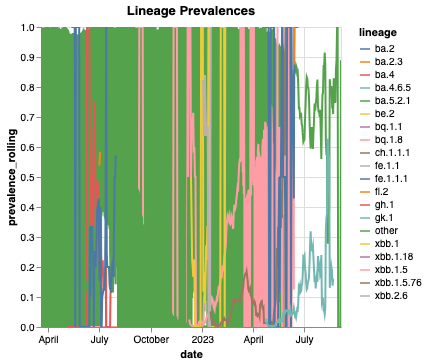
\includegraphics[width=0.8\textwidth]{lineage_viz.png} 
    \caption{Selecting Trending Lineages}
    \label{fig:my_label_2}
\end{figure}
\paragraph{\textbf{}}
\paragraph{We utilized the outbreak package to access up-to-date information regarding virus lineages, mutations, and infection rates. We are doing this project on selected regions noted in the final World Health Organization's weekly viral infection's report, where Sars-CoV-2 levels are rising and intermediate currently (i.e Brazil, Chile, Bolivia). Using this information, along with the available data can help give us a retrospective insight into how the virus became more infectious in these regions to today.To clean the data, we will be checking the data to remove any inconsistencies and handle missing values appropriately. Furthermore, we will analyze the temporal and spatial patterns of virus transmission using various visualization techniques. Conducting exploratory data analysis is essential to gain insight into the distribution of various variables and uncover possible correlations. EDA allows us to examine the patterns, distributions, and relationships within our dataset systematically. This helps identify potential connections between different variables that may be valuable in further analysis or modeling efforts.}
\section{\textbf{Feature Engineering and Selection}}
\paragraph{In our endeavor to understand the transmission dynamics of the SARS-CoV-2 virus, we undertook rigorous feature engineering and selection processes. Our primary objective, as established in our business goals, was to leverage machine learning in identifying mutations that potentially increase transmission rates. This would aid in better forecasting and management of outbreaks.}
\paragraph{\textbf{Feature Engineering}}
\paragraph{\textbf{}}
\begin{figure}[h]
    \centering
    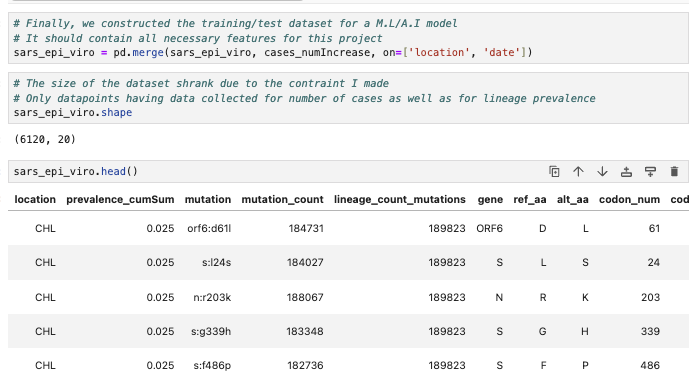
\includegraphics[width=0.8\textwidth]{feature_engineering.png} 
    \caption{Feature Engineering}
    \label{fig:my_label_3}
\end{figure}
\paragraph{Based on the comprehensive insights derived from our exploratory data analysis (EDA), we created new features that could be indicative of a lineage's transmissibility. Most of the features were included in order to capture the essence of how different virus lineages might behave concerning their spread. Different API endpoints returned different features, and we have to collate and merge these along special keys to ensure they tell a story.}
\paragraph{\textbf{}}
\paragraph{\textbf{Feature Selection}}
\paragraph{\textbf{}}
\begin{figure}[h]
    \centering
    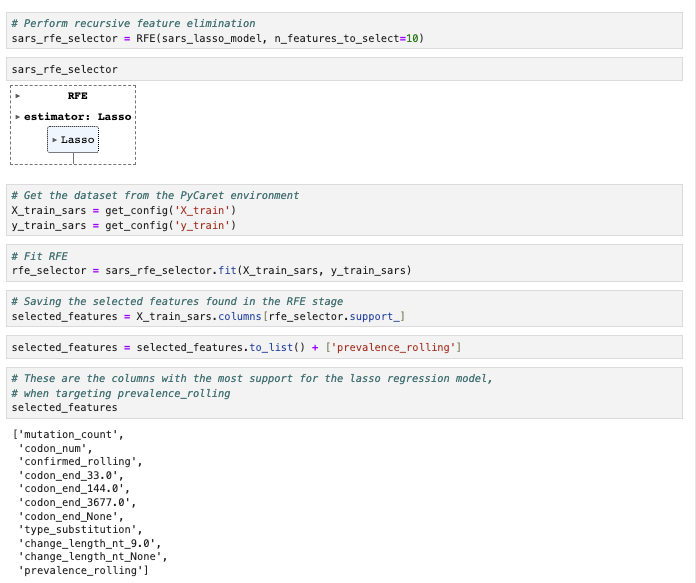
\includegraphics[width=0.8\textwidth]{feature_selection.png} 
    \caption{Feature Selection}
    \label{fig:my_label_4}
\end{figure}
\paragraph{\textbf{}}
\paragraph{To ensure that our machine learning models are fed with the most relevant and impactful information, we employed the recursive feature elimination (RFE) technique. This method helped in narrowing down the most significant features by iteratively removing the least important ones. For this process, we leveraged a model, specifically the LASSO Machine Learning model, to guide the selection.}
\paragraph{\textbf{}}
\begin{figure}[h]
    \centering
    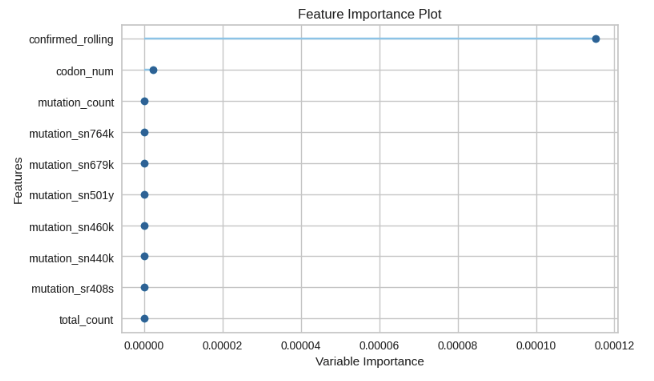
\includegraphics[width=0.8\textwidth]{feature_importance.png} 
    \caption{Feature Importance}
    \label{fig:my_label_5}
\end{figure}
\paragraph{\textbf{}}
\paragraph{Our goal was to enhance the accuracy and robustness of our predictive models, ensuring they provide valuable insights for better pandemic management, by using RFE and LASSO to reduce the number of features used to those that are most important. However, given the evaluation of our model, and the feature's which the model selected as 'important', along with our very small (20 feature) starting shape, we can see that maybe a different model and recursive feature elimination were not needed. Reducing the number of features to only 1 or 2 could be a reason why our model performed so poorly.}
\section{\textbf{Model Selection and Training}}
\paragraph{In the pursuit of discerning the intricacies of virus mutations and their potential to increase transmission rates, we employed the LASSO regression model for our analysis.}
\paragraph{\textbf{}}
\paragraph{\textbf{Why LASSO?}: LASSO (Least Absolute Shrinkage and Selection Operator) regression is renowned for its capacity to perform both variable selection and regularization. This makes it especially apt for scenarios where feature selection is crucial. The inherent regularization in LASSO helps in preventing overfitting, especially when dealing with datasets that have many features. Given our dataset had 20 features before recursive feature elimination, and 11 after, perhaps LASSO would not be the most appropriate given the available data - as it would shrink the number of features used and their relative importance.}
\paragraph{\textbf{}}
\paragraph{\textbf{Data Preparation for Modeling}: Our primary dataset within the project itself, sars epi viro, was meticulously crafted by merging lineage mutations with corresponding infection rate data. This dataset served as the backbone for our model training.}
\paragraph{\textbf{}}
\paragraph{\textbf{Feature Selection}: A noteworthy step in our modeling process was the use of Recursive Feature Elimination (RFE) with the LASSO model. This ensured that we were only using the most relevant features, thereby improving the potential accuracy and interpretability of our model.}
\paragraph{\textbf{}}
\paragraph{\textbf{Model Training}: With the selected features, we trained the LASSO regression model. This model was then primed to predict the association between mutation characteristics and increased transmission rates.}
\paragraph{\textbf{}}
\paragraph{\textbf{Model Evaluation}: Post-training, the model was subjected to a comprehensive evaluation. While the exact metrics and results were not detailed in the extracted sections, it's imperative to understand that such evaluations help in ascertaining the model's performance and its real-world applicability.}
\paragraph{In essence, by leveraging the LASSO regression model, we aim to robustly predict the mutation characteristics that might be strongly correlated with increased virus transmission rates, which is of paramount importance in managing the pandemic more effectively.}
\paragraph{Our choice of model can always be improved, and the best model is always going to be the one that is being continually improved and built upon for the goal in question. }
\section{Final Review: Evaluation  Testing}
\paragraph{\textbf{}}
\begin{figure}[h]
    \centering
    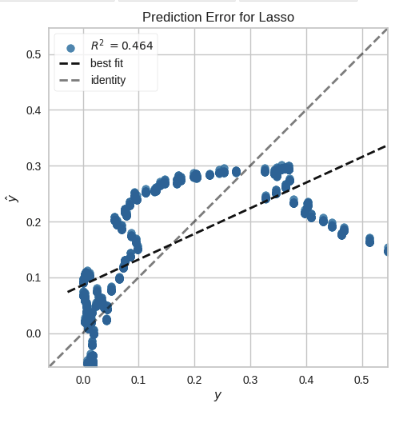
\includegraphics[width=0.8\textwidth]{prediction_error.png} 
    \caption{Plot of Predicted Y versus True Y}
    \label{fig:my_label_6}
\end{figure}
\paragraph{\textbf{}}
\paragraph{As we approached the culmination of our project, we directed our focus toward ensuring that the machine learning model we developed was both accurate and reliable. Our primary objective remained unchanged: to harness the power of machine learning in identifying virus mutations that might lead to heightened transmission rates.}
\paragraph{\textbf{}}
\begin{figure}[h]
    \centering
    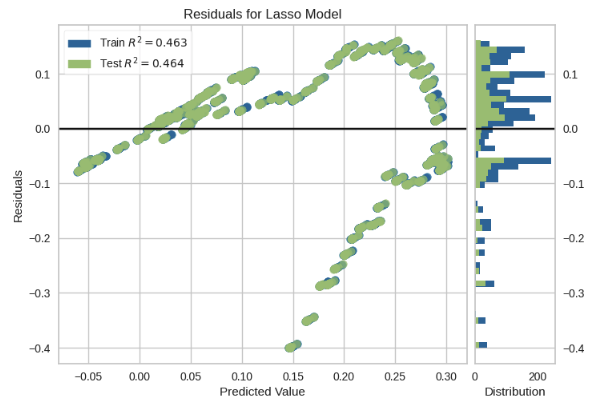
\includegraphics[width=0.8\textwidth]{residuals.png} 
    \caption{Plot of Residuals}
    \label{fig:my_label_7}
\end{figure}
\paragraph{\textbf{}}
\paragraph{\textbf{Model Validation}: To ascertain the efficacy of our model, we employed validation techniques. Cross-validation stood out as our chosen method, renowned for its ability to assess a model's performance on unseen data. By splitting our data multiple times into training and testing sets and evaluating the model's performance across these different splits, we aimed to ensure the robustness of our model and minimize the risk of overfitting.}
\paragraph{\textbf{Documentation and Sharing of Insights}: Recognizing the importance of sharing our findings with the broader community, we have taken steps to document our research comprehensively. A detailed article on Medium was posted here: https://medium.com/@bryanambzam/an-epidemiological-analysis-of-sars-cov-2-using-pycaret-ce6fe1d7c178}
\paragraph{We aim to make the insights more accessible to the general public and the tech community. Furthermore, this research paper was constructed to delve deeper into the technicalities and findings. This paper will be shared with stakeholders, collaborating organizations, and the scientific community at large. We hope that by disseminating our research, we can foster collective efforts in understanding and combating the virus more effectively.}
\section{\textbf{Deployment and Future Work}}
\paragraph{Deploy the trained model to a web application or platform where it can be accessed and utilized by researchers, public health officials, and other relevant parties. The deployment will be available on the GitHub repo here: https://github.com/Bryan-Az/Data-Methods/tree/main/CRISP-DM}
\paragraph{With the ever-evolving landscape of SARS-CoV-2, research continues to shed light on its genetic architecture and transmission dynamics. Recent studies \cite{masahiro_kanai_69ddf437} cover the significance of understanding host genetic factors in determining COVID-19 severity and susceptibility. Through advanced genome-wide association studies, 51 distinct genome-wide significant loci were identified. These loci shed light on major biological pathways involved in susceptibility and severity, including viral entry, airway defense in mucus, and type I interferon.}
\paragraph{Another innovative approach \cite{smruthi_karthikeyan_cd33e450} involves utilizing wastewater sequencing for early detection of emerging variants. Such methods have proven effective in tracking regional infection dynamics, providing a less biased view compared to clinical testing. Moreover, emerging variants were detected up to 14 days earlier in wastewater samples, showcasing the potential of this method for early surveillance.}
\paragraph{With the CRISP-DM methodology guiding our analytical approach, as demonstrated in our recent analysis in the "COVID-Health-BI.ipynb" notebook, the future holds promising milestones for virology and epidemiological studies. As SARS-CoV-2 continues to mutate and spread, integrating insights from clinical, genetic, and wastewater surveillance will be paramount. The convergence of these data streams, facilitated by machine learning and data mining techniques, can enable more accurate forecasting, early detection of high-risk variants, and better pandemic management.}
\paragraph{The multifaceted nature of SARS-CoV-2, combined with its rapid evolution, underscores the need for continuous, integrated research. The virus is not just traveling across geographies but also evolving genetically, demanding our constant vigilance. By harnessing the power of modern research methodologies, data analytics, and collaborative efforts, we can hope to stay a step ahead in our understanding and mitigation strategies. The insights from the recent studies, combined with our analysis, provide a beacon of hope, illuminating the path forward in our collective fight against this pandemic.}
\printbibliography
\end{document}